\part{Some leftovers}
\frame{\partpage}

\begin{frame}{Linear SCMs}
  \begin{Def}
We call an SCM $\C{M}=\langle \Sin, \Send, \Srnd, \CX, P, f \rangle$
\emph{linear} if all variables are real-valued and
each component of the causal mechanism is a linear combination of variables, that is
$$
  f_v(x) = \sum_{w\in V \cup J \cup W} B_{vw} x_w,
$$
where $B\in\RN^{V \times (V \cup J \cup W)}$ is a matrix of coefficients.
  \end{Def}

For any set $L \subseteq V$,
$(\C{M})_{\doit(V\setminus L)}$ is uniquely solvable if and only if the matrix $I_{L}-B_{LL}$ is invertible
(where $I_L \in \RN^{L \times L}$ the identity matrix and $B_{LL} \in \RN^{L \times L}$ the submatrix from $B$).
\end{frame}

\begin{frame}{Hard interventions commute}
In the following slides, we always consider an SCM
$\C{M} = \langle \Sin, \Send, \Srnd, \CX, P, f \rangle$.

\begin{block}{Proposition}
Hard interventions $\doit(T_1\dots)$, $\doit(T_2\dots)$ with disjoint targets $T_1, T_2 \subseteq \Sin \cup \Srnd \cup \Send$ (of any of the three variants) commute:
  $$(\C{M}_{\doit(T_1\dots)})_{\doit(T_2\dots)} = (\C{M}_{\doit(T_2\dots)})_{\doit(T_1\dots)}.$$
\end{block}
Try proving this yourself!
\end{frame}

\begin{frame}{Hard interventions compatible with twinning}
\begin{block}{Proposition}
\begin{itemize}
  \item For $T \subseteq \Sin \cup \Send$, $\xT \in \CXT$:
    $$(\C{M}^\twin)_{\doit(X_T=\xT,X_{T'}=\xT)} = (\C{M}_{\doit(\XT=\xT)})^\twin.$$
  \item For $T \subseteq \Srnd$, $Q_T \in \prod_{t\in T} \C{P}(\CX_t)$:
    $$(\C{M}^\twin)_{\doit(X_T\sim Q_T)} = (\C{M}_{\doit(\XT\sim Q_T)})^\twin.$$
  \item For $T \subseteq \Sin \cup \Send$:
    $$(\C{M}^\twin)_{\doit(T,T')} = (\C{M}_{\doit(T)})^\twin.$$
%  \item If $\C{M}_{\doit(B)}$ is uniquely solvable for $B \subseteq \Send$, then
%    $(\C{M}_B)^\twin \equiv (\C{M}^\twin)_{B\dot\cup B'}$.
\end{itemize}
\end{block}
Try proving this yourself!
\end{frame}

\begin{frame}{Twinning preserves unique solvability and simplicity}    
\begin{Prp}
If $\C{M}$ is uniquely solvable, then $\C{M}^{\twin}$ is uniquely solvable.
Furthermore, if $\C{M}$ is simple, then $\C{M}^{\twin}$ is simple.
\end{Prp}
\begin{proof}
  Explicitly construct the solution function of an intervened $\C{M}^{\twin}$ in terms of that of an intervened $\C{M}$.
  Straightforward, but cumbersome bookkeeping. For details, see lecture notes. 
\end{proof}
\end{frame}

\begin{frame}{Updated definition of observational equivalence}
  Extension for the case $J \ne \tilde{J}$:
  \begin{definition}
  Let $\C{M} = \langle \Sin, \Send, \Srnd, \CX, P, f \rangle$ and
  $\tilde{\C{M}} = \langle \tilde{\Sin}, \tilde{\Send}, \tilde{\Srnd}, \tilde{\CX}, \tilde{P}, \tilde{f} \rangle$ be two simple SCMs
  and $O \subseteq (\Send \cup \Srnd) \cap (\tilde{\Send} \cup \tilde{\Srnd})$ a subset.
  We say that
  $\C{M}$ and $\tilde{\C{M}}$ are \emph{observationally equivalent w.r.t.\ $O$} if $\CX_O = \tilde{\CX}_O$, $\CX_{J \cap \tilde{J}} = \tilde{\CX}_{J \cap \tilde{J}}$ and their marginal Markov kernels coincide:
      $$P_{\C{M}}(X_O \mid \doit(X_J)) = P_{\tilde{\C{M}}}(X_O \mid \doit(X_{\tilde J})).$$
    This has to be interpreted as both Markov kernels being a version of a Markov kernel $\CX_{J \cap \tilde{J}} \dshto \CX_O$,
    i.e., $P_{\C{M}}(X_O \mid \doit(X_J))$ must be essentially constant in $x_{J \setminus \tilde{J}}$ and
    $P_{\tilde{\C{M}}}(X_O \mid \doit(X_{\tilde{J}}))$ must be essentially constant in $x_{\tilde{J} \setminus J}$.
\end{definition}
\end{frame}

\begin{frame}{Application of the updated definition}
\begin{Lem}
Let $\C{M} = \langle \Sin, \Send, \Srnd, \CX, P, f \rangle$ be a simple SCM. Then
$\C{M}$ and $\C{M}^\twin$ are interventionally equivalent w.r.t.\ $V \cup W$.
\end{Lem}
\begin{proof}
  Writing out the definitions with rather cumbersome bookkeeping.
  See lecture notes for details.
\end{proof}
\end{frame}

\part{Marginalizations}
\frame{\partpage}

\begin{frame}{Marginalizations: Motivation}
  Often we like to obtain a simpler description of a system by hiding irrelevant details of a subsystem.

  \begin{block}{Examples}
    \begin{enumerate}
      \item Moving code into a subroutine when programming
      \item Marginalizing a probability distribution over some variables
      \item Taking an orthogonal projection in linear algebra
      \item Taking a latent projection of a CDMG
    \end{enumerate}
  \end{block}

  For SCMs, we define a marginalization over a subset of endogenous variables that removes those
  variables from the model but preserves the causal semantics of the remaining variables.
\end{frame}

\begin{frame}{Marginalizations: Basic insight}
  Write $M := V \setminus L$.
    \begin{equation*}\begin{split}
%  & \begin{cases}
%    x_L = g_L(x_J,x_W) \\
%    x_M = g_M(x_J,x_W) \\
%  \end{cases} \\
%  \iff 
  & \begin{cases}
    x_L = f_L(x_J,x_M,x_L,x_W) \\
    x_M = f_M(x_J,x_M,x_L,x_W) \\
  \end{cases} \\
  \iff & \begin{cases}
    x_L = \tilde{g}_L(x_J,x_M,x_W) \\
    x_M = f_M(x_J,x_M,x_L,x_W) \\
  \end{cases}  \\
  \iff & \begin{cases}
    x_L = \tilde{g}_L(x_J,x_M,x_W) \\
    x_M = f_M(x_J,x_M,\tilde{g}_L(x_J,x_M,x_W),x_W) \\
  \end{cases} \\
  \iff & \begin{cases}
    x_L = \tilde{g}_L(x_J,x_M,x_W) \\
    x_M = \tilde{f}(x_J,x_M,x_W) \\
  \end{cases}
  \end{split}\end{equation*}
  We can now forget $x_L$, and only retain:
  $$x_M = \tilde{f}(x_J,x_M,x_W)$$
\end{frame}

\begin{frame}{Marginalizations: Definition}
\begin{Def}
  Let $L \subseteq \Send$ be such that $\C{M}_{\doit(V\setminus L)}$ is uniquely solvable.
  Write $M = V \setminus L$ and let $\tilde{g}_L : \CX_{\Sin \cup M} \times \CXW \to \CX_L$
  be the unique solution function for $\C{M}_{\doit(M)}$.
  Then we call $\C{M}_{\setminus L} = \langle \Sin, M, \Srnd, \CX_{\Sin} \times \CX_{M} \times \CX_{\Srnd}, P, \tilde{f} \rangle$ with
  $$\tilde{f}(\xJ,x_{M},\xW) = f_{M}(\xJ,x_{M},\tilde{g}_L(\xJ,x_{M},\xW),\xW)$$
  the \emph{marginalization of $\C{M}$ over $L$}.
\end{Def}
\end{frame}

\begin{frame}{Marginalization: Properties I}
In the next three slides, assume that
$L \subseteq \Send$ is such that $\C{M}_{\doit(V \setminus L)}$ is uniquely solvable
(i.e., $\C{M}_{\setminus L}$ is defined).
\begin{Lem}
  If $\C{M}$ is uniquely solvable then 
  \begin{itemize}
    \item its marginalization $\C{M}_{\setminus L}$ is uniquely solvable; 
    \item the unique solution function for $\C{M}_{\setminus L}$ is just $g_{V\setminus L}$, where 
  $g : \CX_J \times \CX_W \to \CX_V$ is the unique solution function for $\C{M}$.
  \end{itemize}
\end{Lem}

This gives:
$$P_{\C{M}_{\setminus L}}(X_{V\setminus L},X_W \mid \doit(X_J)) = P_{\C{M}}(X_{V\setminus L},X_W \mid \doit(X_J))$$
(The Markov kernel of the marginalized SCM is given by the marginal Markov kernel of the SCM).
\end{frame}
  
\begin{frame}{Marginalization: Properties II}
  \begin{Prp}
    For a hard intervention $\doit(T\dots)$ with target $T \subseteq \Sin \cup \Srnd \cup \Send$ (of any of the three variants) such that $L \cap T = \emptyset$:
    $$(\C{M}_{\doit(T\dots)})_{\setminus L} = (\C{M}_{\setminus L})_{\doit(T\dots)}.$$
\end{Prp}
Try proving this yourself!

\begin{Prp}
$$(\C{M}_{\setminus L})^\twin = (\C{M}^\twin)_{\setminus (L\cup L')}.$$
\end{Prp}
Try proving this yourself!
\end{frame}

\begin{frame}{Marginalization: Properties III}
\begin{Prp}
  Let $L_2 \subseteq \Send$ such that $L \cap L_2 = \emptyset$.
  If $(\C{M}_{\setminus L})_{\doit((V\setminus L)\setminus L_2)}$ is uniquely solvable, then $\C{M}_{\doit(V\setminus(L\cup L_2))}$ is uniquely solvable, and:
  $$(\C{M}_{\setminus L})_{\setminus L_2} = \C{M}_{\setminus (L\cup L_2)}.$$
\end{Prp}
\begin{proof}
  Straightforward, but cumbersome notation. See lecture notes.
\end{proof}
\end{frame}

\begin{frame}{Marginalization: Properties for Simple  SCMs}
Let $\C{M} = \langle \Sin, \Send, \Srnd, \CX, P, f \rangle$ be a simple SCM.
\begin{Prp}
  For any $L \subseteq \Send$, the marginalization $\C{M}_{\setminus L}$ is also simple.
\end{Prp}
\begin{proof}
  For $T \subseteq J \cup W \cup V \setminus L$, marginalization commutes with hard intervention:
  $$(\C{M}_{\setminus L})_{\doit(T)} = (\C{M}_{\doit(T)})_{\setminus L}.$$
  Because $\C{M}$ is simple, also $\C{M}_{\doit(T)}$ is simple, and in particular it is
  uniquely solvable. 
  Hence its marginalization $(\C{M}_{\doit(T)})_{\setminus L}$ is uniquely solvable.
  This means that $(\C{M}_{\setminus L})_{\doit(T)}$ is uniquely solvable. Since this
  holds for any $T$, $\C{M}_{\setminus L}$ is simple.
\end{proof}
\begin{Cor}
  For $L_1, L_2 \subseteq \Send$ with $L_1 \cap L_2 = \emptyset$:
    $(\C{M}_{\setminus L_1})_{\setminus L_2} = (\C{M}_{\setminus L_2})_{\setminus L_1} = \C{M}_{\setminus (L_1 \cup L_2)}$.
\end{Cor}
\end{frame}

\begin{frame}{Marginalizations preserve causal semantics}
\begin{Thm}
  Let $\C{M} = \langle \Sin, \Send, \Srnd, \CX, P, f \rangle$ be a simple SCM and $L \subseteq \Send$.
  Then $\C{M}$ and $\C{M}_{\setminus L}$ are observationally,
  interventionally and counterfactually equivalent w.r.t.\ $(V \cup W) \setminus L$.
\end{Thm}
\begin{proof}
  Write $M := V \setminus L$. We already noticed that
  $P_{\C{M}}(X_M,X_W \mid \doit(X_J)) = P_{\C{M}_{\setminus L}}(X_M,X_W \mid \doit(X_J))$.

  Let $T \subseteq M \cup W$. Then $(\C{M}_{\setminus L})_{\doit(T)} = (\C{M}_{\doit(T)})_{\setminus L}$.
  The observational equivalence of $\C{M}_{\doit(T)}$ and $(\C{M}_{\doit(T)})_{\setminus L}$ w.r.t.\ $(M \cup W) \setminus T$ hence implies the observational equivalence of $\C{M}_{\doit(T)}$ and $(\C{M}_{\setminus L})_{\doit(T)}$ w.r.t.\ $(M \cup W) \setminus T$.
  Hence, $\C{M}$ and $\C{M}_{\setminus L}$ are interventionally equivalent w.r.t.\ $M \cup W$.

  Finally, $(\C{M}_{\setminus L})^\twin = (\C{M}^\twin)_{\setminus (L \cup L')}$. Since $\C{M}^\twin$ and its marginalization
  $(\C{M}^\twin)_{\setminus (L \cup L')}$ are interventionally equivalent w.r.t.\ $M \cup M' \cup W$,
  $\C{M}$ and $\C{M}_{\setminus L}$ are counterfactually equivalent w.r.t.\ $M \cup W$.
\end{proof}
\end{frame}

\part{Graphs}
\frame{\partpage}

\begin{frame}{Finally, graphs!}
  We introduce the graph of an SCM with nodes corresponding to the variables and directed edges representing the functional relationships, i.e., the structure of the structural equations.
  
  \begin{Def}
  For $i \in \Sin \cup \Send \cup \Srnd$ and $j \in \Send$, we say that
  \emph{$i$ is a parent of $j$ according to $\C{M}$} if there does not exist a measurable function
  $\tilde f_j : \CX_{(\Sin\cup\Send\cup\Srnd) \setminus \{i\}} \to \CX_j$
  such that for all $x \in \CX$,
  $$x_j = f_j(x) \iff x_j = \tilde f_j(x_{\setminus i}),$$
  where $x_{\setminus i}$ is shorthand for $x_{(\Sin\cup\Send\cup\Srnd)\setminus\{i\}}$.
\end{Def}
  \begin{itemize}
    \item In words: $i$ is parent of $j$ if the causal mechanism for $j$ is not equivalent to one that is constant with respect to its input component $i$.
    \item By definition, exogenous (input and random) variables have no parents.
    \item Note that the parent-relationship is preserved under equivalence.
  \end{itemize}
\end{frame}

\begin{frame}{Graphs: Definition}
  \begin{Def}
  The CDG $\langle \Sin, \Send \cup \Srnd, E \rangle$ with
  input nodes $\Sin$, output nodes $\Send\cup\Srnd$, and
  directed edges
  $$E = \{i \to j : i \in \Sin\cup\Srnd\cup\Send, j\in\Send: \text{$i$ is parent of $j$ according to $\C{M}$}\}$$
  is called the \emph{graph of the SCM $\C{M}$} and will be denoted as $G(\C{M})$.
\end{Def}
  \begin{itemize}
    \item Equivalent SCMs have the same graphs.
    \item Observationally equivalent SCMs may have different graphs.
    \item Interventionally equivalent SCMs may have different graphs.
  \end{itemize}
\end{frame}

\begin{frame}{Example}
  \begin{Eg}
    \begin{itemize}
      \item Consider an SCM $\C{M}$
  with endogenous variables $X,Y$ and exogenous random variable $W$ and structural equations
    $$X = -X^3 + X + W, \qquad Y = \sin(X) - W$$
  \item Its graph is $G(\C{M})$: \\
  \centerline{\begin{tikzpicture}
    \node[var] (W) at (0,0) {$W$};
    \node[var] (X) at (1.5,0) {$X$};
    \node[var] (Y) at (3,0) {$Y$};
    \draw[arr] (W) -- (X);
    \draw[arr,bend left] (W) edge (Y);
    \draw[arr] (X) -- (Y);
  \end{tikzpicture}}
\item Note: $X$ is not a parent to itself, because
  its structural equation is equivalent to $X = \sqrt[3]{W},$
  where $X$ does not appear on the r.h.s..
\item
  When considering exogenous random variables as latent, we can consider the marginalized graph $G(\C{M})^{\setminus W}$:\\

  \medskip
  \centerline{\begin{tikzpicture}
    \node[var] (X) at (1.5,0) {$X$};
    \node[var] (Y) at (3,0) {$Y$};
    \draw[biarr,bend left] (X) edge (Y);
    \draw[arr] (X) -- (Y);
  \end{tikzpicture}}
    \end{itemize}
  \end{Eg}
\end{frame}

\begin{frame}{Example: Self-cycle}
\begin{Eg}
  The graph of an SCM with structural equation
  $$X = W X + c$$
  ($X$ endogenous, $W$ exogenous random) has a \emph{self-cycle} at $X$:\\
  \centerline{\begin{tikzpicture}
    \node[var] (W) at (0,0) {$W$};
    \node[var] (X) at (1.5,0) {$X$};
    \draw[arr] (W) -- (X);
    \draw[arr,in=30,out=-30,looseness=5] (X) edge (X);
  \end{tikzpicture}}
\end{Eg}
Self-cycles are a warning sign of complications with respect to solvability.
They are of no concern when restricting to the class of simple SCMs.
\begin{Prp}
  For $j \in V$, we have that there is a self-cycle $j \to j$ in $G(\C{M})$ if and only if
  $\C{M}_{\doit(V\setminus \{j\})}$ is \emph{not} uniquely solvable.
  In particular, graphs of simple SCMs have no self-cycles.
\end{Prp}
\end{frame}

\begin{frame}{Twinning operation}
Remember: we already provided definitions for hard interventions and marginalizations (latent projections) on graphs.
We can also define a twinning operation on graphs.
\begin{Def}
  Let $G=\langle J,V \cup W,E\rangle$ be a CDG such that $\Pa^G(W) = \emptyset$.

  Write $J' := \{j' : j \in J\}$ and $V' := \{v' : v \in V\}$ for copies of $J$ and $V$.

  The \emph{twinned graph
  $G^{\twin(J,V)}$} is defined as the CDG $\langle J \dot\cup J', V \dot\cup V' \cup W, \tilde{E}\rangle$ with directed edges
  \begin{equation*}\begin{split}
    \tilde{E} := E & \cup \{w \to v' : w \in W, v \in V, w \to v \in E\} \\
                 & \cup \{i' \to v' : i \in J \cup V, v \in V, i \to v \in E\}.
  \end{split}\end{equation*}
\end{Def}
In words, we copy the nodes $J \cup V$ (but not the nodes $W$) and copy the edges accordingly.
\end{frame}

\begin{frame}{Compatibility of operations on SCMs and graphs}
  \begin{Prp}
  \begin{itemize}
    \item Hard interventions: for $T \subseteq J \cup V \cup W$,
      $$G(\C{M}_{\doit(T)}) = G(\C{M})_{\doit(T)}.$$
    \item Twinning:
      $$G(\C{M})^{\twin(J\cup V)} = G(\C{M}^\twin).$$
    \item Marginalizations: If $\C{M}$ is simple, then for $L \subseteq V$,
      $$G(\C{M}_{\setminus L}) \subseteq G(\C{M})^{\setminus L}.$$
  \end{itemize}
\end{Prp}
\begin{proof}
Try proving the first two statements yourself!
The last statement is more involved. For a proof by induction, see the lecture notes.
\end{proof}
\end{frame}

\begin{frame}{Acyclic SCMs}
\begin{Def}
  An SCM $\C{M}$ is called \emph{acyclic} if its graph $G(\C{M})$ is acyclic.
\end{Def}
  While most literature only considers acyclic SCMs (or CBNs), we propose to
  use simple SCMs instead if one cannot rule out a priori the possibility of causal cycles.
\begin{Prp}
  Acyclic SCMs are simple.
\end{Prp}
\begin{proof}
  Main idea: Choose a topological ordering and solve the system of structural equations in that order.
  For details, see lecture notes.
\end{proof}
\end{frame}

\begin{frame}{Relations between causal models}
  \centerline{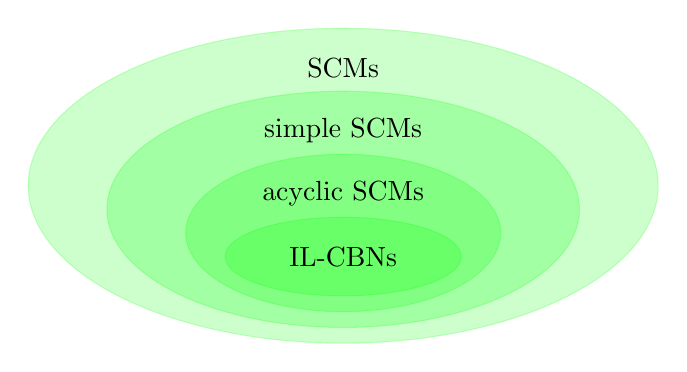
\begin{tikzpicture}
      \begin{scope}
        \draw[draw=green,fill=green,opacity=0.2] (0,0) ellipse (1.5cm and 0.5cm);
        \draw[draw=green,fill=green,opacity=0.2] (0,0.3) ellipse (2cm and 1cm);
        \draw[draw=green,fill=green,opacity=0.2] (0,0.6) ellipse (3cm and 1.5cm);
        \draw[draw=green,fill=green,opacity=0.2] (0,0.9) ellipse (4cm and 2cm);
        \node at (0,0) {IL-CBNs};
        \node at (0,0.8) {acyclic SCMs};
        \node at (0,1.6) {simple SCMs};
        \node at (0,2.4) {SCMs};
      \end{scope}
  \end{tikzpicture}}

  \bigskip
  Simple SCMs are more expressive than IL-CBNs, because they:
  \begin{enumerate}
    \item Encode counterfactuals
    \item Can model causal cycles (e.g., feedback loops)
  \end{enumerate}

  In the next part, we will extend the acyclic causal reasoning theory (global Markov property, do-calculus,
  adjustment) to simple SCMs.
\end{frame}

\part{$\sigma$-Separation and Acyclifications}
\frame{\partpage}

\frame{\frametitle{$\sigma$-Blocking and $\sigma$-Separation}
Remember: $\Sc^G(v) := \Anc^G(v) \cap \Desc^G(v)$.
\begin{definition}
  Let $G = \langle J,E,V,L \rangle$ be a CDMG and $C \subseteq J \cup V$ a subset of nodes and $\pi$ a walk in $G$:
  $$\pi = v_0 \sts \dots \sts v_n.$$
  $\pi$ called \emph{$C$-$\sigma$-blocked}, or \emph{$\sigma$-blocked by $C$}, iff
  \begin{itemize}
    \item $v_0 \in C$ or $v_n \in C$, or
    \item it contains a collider $v_{k-1} \sto v_k \ots v_{k+1}$ with $v_k \not\in C$, or
    \item it contains a non-collider
      $v_{k-1} \sts v_k \to v_{k+1}$  with $v_k \in C$
    \alert{and such that $v_{k+1} \notin \Sc^{G}(v_k)$}, or
    \item it contains a non-collider
      $v_{k-1} \ot  v_k \sts v_{k+1}$ with $v_k \in C$
    \alert{and such that $v_{k-1} \notin \Sc^{G}(v_k)$}.
  \end{itemize}
  We say that \emph{$A$ is $\sigma$-separated from $B$ by $C$}, denoted \emph{$A \Perp^{\alert{\sigma}}_G B \mid C$}, if every walk with one end node in $A$ and one end node in $B \cup J$ is $\sigma$-blocked by $C$.
\end{definition}
}

\frame{\frametitle{Example: $\sigma$-Separation}
\begin{example}
  \begin{tikzpicture}
      \node at (1,3.5) {Graph $G(\C{M})$:};
      \node[var] (X1) at (0,0) {$X_1$};
      \node[var] (X2) at (1.5,0) {$X_2$};
      \node[var] (X3) at (1.5,1.5) {$X_3$};
      \node[var] (X4) at (0,1.5) {$X_4$};
      \node[varh] (W1) at (-1,-1) {$W_1$};
      \node[varh] (W2) at (2.5,-1) {$W_2$};
      \node[varh] (W3) at (2.5,2.5) {$W_3$};
      \node[varh] (W4) at (-1,2.5) {$W_4$};
      \draw[arr] (X1) edge (X2);
      \draw[arr] (X2) edge (X3);
      \draw[arr] (X3) edge (X4);
      \draw[arr] (X4) edge (X1);
      \draw[arrh] (W1) edge (X1);
      \draw[arrh] (W2) edge (X2);
      \draw[arrh] (W3) edge (X3);
      \draw[arrh] (W4) edge (X4);
      \node at (-3,3.5) {SCM $\C{M}$:};
      \node[text width=4cm] at (-3,1) {\small $X_1=X_4+W_1$\\
      $X_2=X_1 \cdot W_2$\\
      $X_3=X_2+W_3$\\
      $X_4=X_3\cdot W_4$};
      \node at (5,1.75) {$X_1 \displaystyle\Perp^d X_3 \given X_2, X_4$};
      \node at (5,1) {but};
      \node at (5,0.25) {$X_1 \displaystyle\nPerp^\sigma X_3 \given X_2, X_4$};
  \end{tikzpicture}
\end{example}

\bigskip
In general: No $\sigma$-separations between nodes within the same strongly connected component.
}

\begin{frame}{Graphical Acyclifications: Definition}
\begin{Def}
  Given a CDMG $G = \langle J, V, E, L \rangle$, we call a CADMG $G' = \langle J, V, E', L' \rangle$
  an \emph{acyclification of $G$} if
  \begin{enumerate}
    \item $G'$ is acyclic;
    \item $G'$ has the same input nodes $J$ and output nodes $V$ as $G$;
    \item for any pair of nodes $\{i,j\}$ such that $i \not\in\Sc^G(j)$:
      \begin{enumerate}
      \item $i \to j \in E'$ iff there exists a node $j' \in \Sc^G(j)$ such that $i \to j' \in E$;
      \item $i \oto j \in L'$ iff there exist nodes $i' \in \Sc^G(i), j' \in \Sc^G(j)$ such that $i' \oto j' \in L$;
      \end{enumerate}
    \item for any pair of distinct nodes $\{i,j\}$ such that $i \in\Sc^G(j)$: $i \to j \in E'$ or $i \ot j \in E'$ or $i \oto j \in L'$.
  \end{enumerate}
\end{Def}
\end{frame}

\begin{frame}{Graphical Acyclifications: Example}
  \scalebox{0.8}{\begin{tikzpicture}
    \begin{scope}
      \node at (1.5,2) {Graph:};
      \node[varh] (W1) at (1,1) {$W_1$};
      \node[varh] (W2) at (2,1) {$W_2$};
      \node[varh] (W3) at (1,0) {$W_3$};
      \node[varh] (W4) at (2,0) {$W_4$};
      \node[varh] (W5) at (1,-2) {$W_5$};
      \node[varh] (W6) at (2,-2) {$W_6$};
      \node[var] (X1) at (0,0) {$X_1$};
      \node[var] (X2) at (3,0) {$X_2$};
      \node[var] (X3) at (0,-1) {$X_3$};
      \node[var] (X4) at (3,-1) {$X_4$};
      \node[var] (X5) at (0,-2) {$X_5$};
      \node[var] (X6) at (3,-2) {$X_6$};
      \draw[arrh] (W1) -- (X1);
      \draw[arrh] (W2) -- (X2);
      \draw[arrh] (W3) -- (X3);
      \draw[arrh] (W4) -- (X4);
      \draw[arrh] (W5) -- (X5);
      \draw[arrh] (W6) -- (X6);
      \draw[arr] (X1) -- (X3);
      \draw[arr] (X2) -- (X4);
      \draw[arr] (X3) -- (X5);
      \draw[arr] (X4) -- (X6);
      \draw[arr,bend left=20] (X3) edge (X4);
      \draw[arr,bend left=20] (X4) edge (X3);
    \end{scope}
    \begin{scope}[yshift=-5cm,xshift=-5cm]
      \node[varh] (W1) at (1,1) {$W_1$};
      \node[varh] (W2) at (2,1) {$W_2$};
      \node[varh] (W3) at (1,0) {$W_3$};
      \node[varh] (W4) at (2,0) {$W_4$};
      \node[varh] (W5) at (1,-2) {$W_5$};
      \node[varh] (W6) at (2,-2) {$W_6$};
      \node[var] (X1) at (0,0) {$X_1$};
      \node[var] (X2) at (3,0) {$X_2$};
      \node[var] (X3) at (0,-1) {$X_3$};
      \node[var] (X4) at (3,-1) {$X_4$};
      \node[var] (X5) at (0,-2) {$X_5$};
      \node[var] (X6) at (3,-2) {$X_6$};
      \draw[arrh] (W1) -- (X1);
      \draw[arrh] (W2) -- (X2);
      \draw[arrh] (W3) -- (X3);
      \draw[arrh] (W4) -- (X4);
      \draw[arrh] (W3) -- (X4);
      \draw[arrh] (W4) -- (X3);
      \draw[arrh] (W5) -- (X5);
      \draw[arrh] (W6) -- (X6);
      \draw[arr] (X1) -- (X3);
      \draw[arr] (X2) -- (X4);
      \draw[arr] (X1) edge (X4);
      \draw[arr] (X2) edge (X3);
      \draw[arr] (X3) -- (X4);
      \draw[arr] (X3) -- (X5);
      \draw[arr] (X4) -- (X6);
    \end{scope}
    \begin{scope}[yshift=-5cm]
      \node at (1.5,2) {Various acyclifications:};
      \node[varh] (W1) at (1,1) {$W_1$};
      \node[varh] (W2) at (2,1) {$W_2$};
      \node[varh] (W3) at (1,0) {$W_3$};
      \node[varh] (W4) at (2,0) {$W_4$};
      \node[varh] (W5) at (1,-2) {$W_5$};
      \node[varh] (W6) at (2,-2) {$W_6$};
      \node[var] (X1) at (0,0) {$X_1$};
      \node[var] (X2) at (3,0) {$X_2$};
      \node[var] (X3) at (0,-1) {$X_3$};
      \node[var] (X4) at (3,-1) {$X_4$};
      \node[var] (X5) at (0,-2) {$X_5$};
      \node[var] (X6) at (3,-2) {$X_6$};
      \draw[arrh] (W1) -- (X1);
      \draw[arrh] (W2) -- (X2);
      \draw[arrh] (W3) -- (X3);
      \draw[arrh] (W4) -- (X4);
      \draw[arrh] (W3) -- (X4);
      \draw[arrh] (W4) -- (X3);
      \draw[arrh] (W5) -- (X5);
      \draw[arrh] (W6) -- (X6);
      \draw[arr] (X1) -- (X3);
      \draw[arr] (X2) -- (X4);
      \draw[arr] (X1) edge (X4);
      \draw[arr] (X2) edge (X3);
      \draw[arr] (X4) -- (X3);
      \draw[arr] (X3) -- (X5);
      \draw[arr] (X4) -- (X6);
    \end{scope}
    \begin{scope}[yshift=-5cm,xshift=5cm]
      \node[varh] (W1) at (1,1) {$W_1$};
      \node[varh] (W2) at (2,1) {$W_2$};
      \node[varh] (W3) at (1,0) {$W_3$};
      \node[varh] (W4) at (2,0) {$W_4$};
      \node[varh] (W5) at (1,-2) {$W_5$};
      \node[varh] (W6) at (2,-2) {$W_6$};
      \node[var] (X1) at (0,0) {$X_1$};
      \node[var] (X2) at (3,0) {$X_2$};
      \node[var] (X3) at (0,-1) {$X_3$};
      \node[var] (X4) at (3,-1) {$X_4$};
      \node[var] (X5) at (0,-2) {$X_5$};
      \node[var] (X6) at (3,-2) {$X_6$};
      \draw[arrh] (W1) -- (X1);
      \draw[arrh] (W2) -- (X2);
      \draw[arrh] (W3) -- (X3);
      \draw[arrh] (W4) -- (X4);
      \draw[arrh] (W3) -- (X4);
      \draw[arrh] (W4) -- (X3);
      \draw[arrh] (W5) -- (X5);
      \draw[arrh] (W6) -- (X6);
      \draw[arr] (X1) -- (X3);
      \draw[arr] (X2) -- (X4);
      \draw[arr] (X1) edge (X4);
      \draw[arr] (X2) edge (X3);
      \draw[biarr] (X4) -- (X3);
      \draw[arr] (X3) -- (X5);
      \draw[arr] (X4) -- (X6);
    \end{scope}
  \end{tikzpicture}}
\end{frame}

\begin{frame}{Graphical Acyclifications: Purpose}
The important property of acyclifications is that they can be used to express $\sigma$-separation in a (possibly cyclic) graph
in terms of $d$-separation in an acyclification.
\begin{Prp}
  Let $G = \langle J, V, E, L \rangle$ be a CDMG and $G' = \langle J, V, E', L' \rangle$ an acyclification of $G$.
  Then for $A, B, C \subseteq V \cup J$ (not necessarily disjoint) subsets of nodes,
  $$A \Perp^\sigma_G B \given C \iff A \Perp^\sigma_{G'} B \given C \iff A \Perp^d_{G'} B \given C$$
\end{Prp}
\begin{proof}
  Requires constructing $\sigma$-open paths in $G'$ from those in $G$, and vice versa. 
  See lecture notes.
\end{proof}
\end{frame}

\begin{frame}{Acyclification of SCM: Definition}
  \begin{Def}
  Let $\C{M} = \langle \Sin, \Send, \Srnd, \CX, P, f \rangle$ be a simple SCM with graph $G = G(\C{M})$.
  For each strongly connected component $C$ of $G(\C{M})$ (i.e., a set of the form
  $\Sc^G(v)$ for $v \in \Send$), let
  $g_C : \CX_{\Sin \cup (\Send \setminus C) \cup \Srnd} \to \CX_C$
  be the unique solution function for $\C{M}_{\doit(\Send \setminus C)}$.
  Define $\tilde{f} : \CXJ \times \CXV \times \CXW \to \CXV$ by its components
  $$\tilde{f}_v(\xJ,\xV,\xW) = (g_{\Sc^G(v)})_v(\xJ,x_{\Send\setminus C},\xW)$$
  for $v \in V$.
  $\C{M}^\acy = \langle \Sin, \Send, \Srnd, \CX, P, \tilde{f} \rangle$ is called the
  \emph{acyclification of $\C{M}$}.
\end{Def}
\end{frame}

\begin{frame}{Acyclification of SCM: Purpose}
  \begin{Prp}
    The acyclification $\C{M}^\acy$ of a simple SCM $\C{M}$ is acyclic, observationally equivalent to $\C{M}$,
    and $G(\C{M}^\acy) \subseteq G'$ for any acyclification $G'$ of $G(\C{M})$.
  \end{Prp}
  \begin{proof}
    By example. For a formal proof, see lecture notes.
    \begin{wrapfigure}{r}{0.4\linewidth}
    \scalebox{0.8}{\begin{tikzpicture}
      \begin{scope}
        \node[varh] (W1) at (1,1) {$W_1$};
        \node[varh] (W2) at (2,1) {$W_2$};
        \node[varh] (W3) at (1,0) {$W_3$};
        \node[varh] (W4) at (2,0) {$W_4$};
        \node[var] (X1) at (0,0) {$X_1$};
        \node[var] (X2) at (3,0) {$X_2$};
        \node[var] (X3) at (0,-1) {$X_3$};
        \node[var] (X4) at (3,-1) {$X_4$};
        \draw[arrh] (W1) -- (X1);
        \draw[arrh] (W2) -- (X2);
        \draw[arrh] (W3) -- (X3);
        \draw[arrh] (W4) -- (X4);
        \draw[arr] (X1) -- (X3);
        \draw[arr] (X2) -- (X4);
        \draw[arr,bend left] (X3) edge (X4);
        \draw[arr,bend left] (X4) edge (X3);
      \end{scope}
      \begin{scope}[yshift=-3cm]
        \node[varh] (W1) at (1,1) {$W_1$};
        \node[varh] (W2) at (2,1) {$W_2$};
        \node[varh] (W3) at (1,0) {$W_3$};
        \node[varh] (W4) at (2,0) {$W_4$};
        \node[var,fill=red] (X1) at (0,0) {$X_1$};
        \node[var,fill=green] (X2) at (3,0) {$X_2$};
        \node[var,fill=blue] (X3) at (0,-1) {$X_3$};
        \node[var,fill=blue] (X4) at (3,-1) {$X_4$};
        \draw[arrh] (W1) -- (X1);
        \draw[arrh] (W2) -- (X2);
        \draw[arrh] (W3) -- (X3);
        \draw[arrh] (W4) -- (X4);
        \draw[arrh] (W3) -- (X4);
        \draw[arrh] (W4) -- (X3);
        \draw[arr] (X1) -- (X3);
        \draw[arr] (X2) -- (X4);
        \draw[arr] (X1) edge (X4);
        \draw[arr] (X2) edge (X3);
      \end{scope}
    \end{tikzpicture}}
  \end{wrapfigure}
  Structural equations:
  \begin{align*}
    X_1 &= W_1 \qquad X_3 = X_1 X_4 + W_3 \\
    X_2 &= W_2 \qquad X_4 = X_2 X_3 + W_4
  \end{align*}
  Acyclification:
  \begin{align*}
    &{\color{red}X_1} = W_1 \qquad {\color{blue}X_3} = \frac{W_3 + {\color{red}X_1} W_4}{1 - {\color{red}X_1} {\color{green}X_2}} \\
    &{\color{green}X_2} = W_2 \qquad {\color{blue}X_4} = \frac{{\color{green}X_2} W_3 + W_4}{1 - {\color{red}X_1} {\color{green}X_2}}
  \end{align*}
  \end{proof}
\end{frame}

\part{Global Markov Property}
\frame{\partpage}

\begin{frame}{Global Markov Property for Simple SCMs}
  With the help of the acyclification, we immediately derive a Markov property for simple SCMs from the one for causal Bayesian networks:
  \begin{Cor}
  Let $\C{M} = \langle \Sin, \Send, \Srnd, \CX, P, f \rangle$ be a simple SCM with graph $G = G(\C{M})$
  and observational Markov kernel $P_{\C{M}}(X_V,X_W \given \doit(X_J))$.
  Then for all $A, B, C \ins J \cup V \cup W$ (not necessarily disjoint) we have the implication:
  $$A \Perp^\sigma_{G(\C{M})} B \given C \implies X_A \Indep_{P_{\C{M}}(X_V,X_W \given \doit(\XJ))} X_B \given X_C.$$
  If one wants to make the implicit dependence on $J$ more explicit one can equivalently also write:
    $$A \Perp^\sigma_{G(\C{M})} J \cup B \given C \implies X_A \Indep_{P_{\C{M}}(X_V,X_W \given \doit(\XJ))} X_J,X_B \given X_C.$$
\end{Cor}
\end{frame}
\begin{frame}{Proof of Global Markov Property for Simple SCMs}
\begin{proof}
  \setlength\abovedisplayskip{10pt}
  \setlength\belowdisplayskip{0pt}
  Choose an acyclification $G'$ of $G(\C{M})$. Then:
  \begin{align*}
    A \Perp^\sigma_{G(\C{M})} B \given C &\stackrel{1}{\iff} A \Perp^d_{G'} B \given C \\
    &\stackrel{2}{\implies} A \Perp^d_{G(\C{M}^\acy)} B \given C \\
    &\stackrel{3}{\implies} X_A \Indep_{P_{\C{M}^{\acy}}(X_V,X_W \given \doit(\XJ))} X_B \given X_C \\
    &\stackrel{4}{\iff} X_A \Indep_{P_{\C{M}}(X_V,X_W \given \doit(\XJ))} X_B \given X_C.
  \end{align*}
  \begin{enumerate}
    \item $G'$ is an acyclification of $G(\C{M})$; 
    \item $G(\C{M}^\acy) \subseteq G'$, removing edges preserves $d$-separations; 
    \item the GMP for $\C{M}^\acy$ interpreted as a causal Bayesian network;
    \item $\C{M}^\acy$ is observationally equivalent to $\C{M}$.
  \end{enumerate}
\end{proof}
\end{frame}

\part{Do-Calculus}
\frame{\partpage}

\begin{frame}{Notation}
  \begin{enumerate}
    \item Let $\C{M} = \langle \Sin, \Send, \Srnd, \CX, P, f \rangle$ be a simple SCM;
    \item To model hard interventions $\doit(B)$ for $B \subseteq V \cup W$, introduce \emph{intervention variable} $I_B$;
    \item Extended SCM $\tilde{\C{M}} = \langle \Sin \cup \{I_B\}, \Send, \Srnd, \CX \times (\CX_B \dot\cup \{\star\}), P, \tilde{f} \rangle$ with causal mechanism
$$\tilde{f}(x,x_{I_B}) := \begin{cases}
  f(x) & x_{I_B} = \star \\
  (f_{\setminus B}(x), x_{I_B}) & x_{I_B} \in \CX_B
\end{cases}$$
    \item $x_{I_B} = \star$ encodes that there is no intervention on $B$,\\
while $x_{I_B} \ne \star$ encodes that the hard intervention $\doit(X_B = x_{I_B})$ is performed.
\item The graph of $\tilde{\C{M}}$, $G_{\doit(I_B)}$, has an additional variable $I_B$ with no incoming edges
  and outgoing edges to all $b \in B$.
  \end{enumerate}
%In the do-calculus, we make use of the extended graph $G_{\doit(I_B)}$ to test the separation statement, while the conclusion
%about the existence and identity of particular Markov kernels concerns those of the original SCM $\C{M}$.
\end{frame}

\begin{frame}{Reminder: Notation of Markov kernels}
  For a simple SCM $\C{M}$:
  \begin{enumerate}
    \item Its \emph{observational Markov kernel} is denoted $P_{\C{M}}(X_{V\cup W} \mid \doit(X_J))$.
    \item For a subset $T \subseteq V \cup W$, we write the \emph{interventional Markov kernel}
$$P_{\C{M}}(X_{(V\cup W)\setminus T} \mid \doit(X_J,X_T)) = P_{\C{M}_{\doit(T)}}(X_{(V\cup W)\setminus T} \mid \doit(X_J,X_T)).$$
\item By conditioning on a subset $S \subseteq (V \cup W) \setminus T$, we obtain the conditional interventional Markov kernel
$$P_{\C{M}}(X_{(V\cup W)\setminus (T \cup S)} \mid \doit(X_J,X_T), X_S).$$
  \end{enumerate}
\end{frame}

\begin{frame}{Do-Calculus for simple SCMs (on one slide!)}
  Let $A,B,C \ins V \cup W$ and $D \ins V \cup W \cup J$ be such that $A,B,C,D$ are pairwise disjoint.
  \begin{enumerate}
    \item \emph{Insertion/deletion of observation}: 
      $A \Perp^\sigma_{G_{\doit(D)}} B \given C \cup D$ implies
      \[ P_{\C{M}}\lp X_A|X_B,X_C,\doit(X_{D\cup J})\rp = P_{\C{M}}\lp X_A|X_C,\doit(X_D)\rp.\]
    \item \emph{Action/observation exchange}: $A \Perp^\sigma_{G_{\doit(I_B,D)}} I_B \given B \cup C \cup D$ implies
      \[ P_{\C{M}}\lp X_A|\doit(X_B),X_C,\doit(X_D)\rp  =  P_{\C{M}}\lp X_A|X_B,X_C,\doit(X_D)\rp.\]
    \item \emph{Insertion/deletion of action}: $A \Perp^\sigma_{G_{\doit(I_B,D)}} I_B \given C  \cup D$ implies
      \[ P_{\C{M}}\lp X_A|\doit(X_B),X_C,\doit(X_{D\cup J})\rp = P_{\C{M}}\lp X_A|X_C,\doit(X_{D})\rp.\]
  \end{enumerate}
  Note: all kernels should be interpreted as $\CX_{J \cup \dots} \dshto \dots$, but some are constant in $x_J$!
\end{frame}

\begin{frame}{Proof}
  \begin{proof}
    Same proof as do-calculus for IL-CBNs, except that all $d$-separations need to be replaced with $\sigma$-separations,
    and we invoke the GMP for simple SCMs rather than the GMP for IL-CBNs.
  \end{proof}
\end{frame}

\part{Adjustment}
\frame{\partpage}

\begin{frame}{Adjustment formula for simple SCMs}
Same notation as for do-calculus. Now assume $J \subseteq D$.
\begin{block}{Problem setting}
We want to estimate the \emph{conditional causal effect}
$P_{\C{M}}(X_A|X_C,\doit(X_B,X_D))$
from
$P_{\C{M}}(X_A,X_B,X_F|X_C,\doit(X_D)).$
\end{block}
The following (pairwise disjoint) index sets have the following roles:\\
\begin{description}\small
  \item[$A$]: the outcome variables of interest.
  \item[$B$]: the treatment or intervention variables.
  \item[$C$]: general conditional (context) variables under which the data was collected.
  \item[$D$]: general interventional (context) variables that were set by the experimenter, $J \ins D$.
  \item[$F_0$]: core adjustment variables, i.e.\ features that were measured.
  \item[$F_1$]: additional measured adjustment variables, with $F = F_0 \cup F_1$.
  \item[$H$]: additional unobserved variables.
\end{description}
\end{frame}

\begin{frame}{General adjustment formula for simple SCMs}
  \begin{Thm}
    Assume that all the following conditions hold in the graph $G_{\doit(I_B,D)}$:
    \begin{align}
        (F_0 \cup H) & \Perp^\sigma_{G_{\doit(I_B,D)}} I_B \given (C \cup D), \\
        A & \Perp^\sigma_{G_{\doit(I_B,D)}} (F_1 \cup I_B) \given (B \cup F_0 \cup H \cup C \cup D), \\
                      H &\Perp^\sigma_{G_{\doit(I_B,D)}} B \given (F \cup C \cup  I_B \cup D).
    \end{align}
Then we have the adjustment formula:\small
    \[ P_{\C{M}}(X_A|X_C,\doit(X_B,X_D)) \stackrel{\text{a.s.}}{=}
    P_{\C{M}}(X_A|X_B,X_C,X_F,\doit(X_D)) \circ P_{\C{M}}(X_F|X_C,\doit(X_D))
\]
\end{Thm}
\begin{proof}
  Analogous to that for IL-CBNs, but now use GMP for simple SCMs and replace all d-separations with $\sigma$-separations.
\end{proof}

\end{frame}

\part{Examples of cyclic SCMs}
\frame{\partpage}

\begin{frame}{Modeling feedback loops}
  \begin{itemize}
    \item Feedback loops are often present in systems;
    \item Such systems are usually described as a system of (random) differential equations;
  \end{itemize}

The \emph{equilibrium} states of such systems can often be causally modelled by a (cyclic) SCM.

\bigskip
We consider two examples:
  \begin{enumerate}
    \item Damped coupled harmonic oscillator (simple SCM)
    \item Price-supply-demand (non-simple SCM)
  \end{enumerate}
\end{frame}

\begin{frame}{Example I: Damped Coupled Harmonic Oscillator}
  \centerline{\scalebox{0.8}{\begin{tikzpicture}
    \begin{scope}
      \fill[pattern=north east lines,draw=none] (-1,-1) rectangle (0,1);
      \draw (0,-1) -- (0,1);
      \begin{scope}[yshift=5mm]
      \node (Q1) at (2,0) {$m_1$};
      \node (Q2) at (4,0) {$m_2$};
      \node (Q3) at (6,0) {$m_3$};
      \node (Q4) at (8,0) {$m_4$};
      \node (Q5) at (10,0) {$m_5$};
      \end{scope}
      \begin{scope}[yshift=-5mm]
        \node (l0) at (1,0) {$\ell_0$};
        \node (l1) at (3,0) {$\ell_1$};
        \node (l2) at (5,0) {$\ell_2$};
        \node (l3) at (7,0) {$\ell_3$};
        \node (l4) at (9,0) {$\ell_4$};
        \node (l5) at (11,0) {$\ell_5$};
      \end{scope}
      \fill[black] (2,0) circle (.2);
      \fill[black] (4,0) circle (.2);
      \fill[black] (6,0) circle (.2);
      \fill[black] (8,0) circle (.2);
      \fill[black] (10,0) circle (.2);
      \draw (12,-1) -- (12,1);
      \fill[pattern=north east lines,draw=none] (12,-1) rectangle (13,1);
      \draw[thick,decorate,decoration={coil,aspect=0.7,amplitude=4,segment length=3mm}] (0,0) -- (2,0);
      \draw[thick,decorate,decoration={coil,aspect=0.7,amplitude=4,segment length=3mm}] (2,0) -- (4,0);
      \draw[thick,decorate,decoration={coil,aspect=0.7,amplitude=4,segment length=3mm}] (4,0) -- (6,0);
      \draw[thick,decorate,decoration={coil,aspect=0.7,amplitude=4,segment length=3mm}] (6,0) -- (8,0);
      \draw[thick,decorate,decoration={coil,aspect=0.7,amplitude=4,segment length=3mm}] (8,0) -- (10,0);
      \draw[thick,decorate,decoration={coil,aspect=0.7,amplitude=4,segment length=3mm}] (10,0) -- (12,0);
      \node at (0,1.3) {\tiny $Q_0$};
      \node at (12,1.3) {\tiny $Q_6$};
    \end{scope}
  \end{tikzpicture}}}

Dynamics:
$$ \frac{d^2Q_i}{dt^2} = \frac{k_i}{m_i} (Q_{i+1} - Q_i - \ell_i) + \frac{k_{i-1}}{m_i} (Q_{i-1} - Q_i + \ell_{i-1}) -\frac{b_i}{m_i} \frac{dQ_i}{dt} \qquad i=1,\dots,d.  $$
\pause
At equilibrium (set $\frac{d^2Q_i}{dt^2} = \frac{d Q_i}{dt} = 0$ and solve each equation for $Q_i$):
$$Q_i = \frac{k_i(Q_{i+1} - \ell_i) + k_{i-1}(Q_{i-1}+\ell_{i-1})}{k_i + k_{i-1}} \qquad i=1,\dots,d.$$

  \centerline{\scalebox{0.8}{\begin{tikzpicture}
    \begin{scope}[yshift=-3cm]
      \node[varc] (Q0) at (0,0) {$Q_0$};
      \node[var] (Q1) at (2,0) {$Q_1$};
      \node[var] (Q2) at (4,0) {$Q_2$};
      \node[var] (Q3) at (6,0) {$Q_3$};
      \node[var] (Q4) at (8,0) {$Q_4$};
      \node[var] (Q5) at (10,0) {$Q_5$};
      \node[varc] (Q6) at (12,0) {$Q_6$};
      \node[varc] (K0) at (1,1) {$k_0$};
      \node[varc] (K1) at (3,1) {$k_1$};
      \node[varc] (K2) at (5,1) {$k_2$};
      \node[varc] (K3) at (7,1) {$k_3$};
      \node[varc] (K4) at (9,1) {$k_4$};
      \node[varc] (K5) at (11,1) {$k_5$};
      \node[varc] (L0) at (1,-1) {$\ell_0$};
      \node[varc] (L1) at (3,-1) {$\ell_1$};
      \node[varc] (L2) at (5,-1) {$\ell_2$};
      \node[varc] (L3) at (7,-1) {$\ell_3$};
      \node[varc] (L4) at (9,-1) {$\ell_4$};
      \node[varc] (L5) at (11,-1) {$\ell_5$};
      \draw[arr] (Q0) to (Q1);
      \draw[arr,bend left=20] (Q1) to (Q2);
      \draw[arr,bend left=20] (Q2) to (Q3);
      \draw[arr,bend left=20] (Q3) to (Q4);
      \draw[arr,bend left=20] (Q4) to (Q5);
      \draw[arr,bend left=20] (Q5) to (Q4);
      \draw[arr,bend left=20] (Q4) to (Q3);
      \draw[arr,bend left=20] (Q3) to (Q2);
      \draw[arr,bend left=20] (Q2) to (Q1);
      \draw[arr] (Q6) to (Q5);
      \draw[arr] (K0) -- (Q1);
      \draw[arr] (K1) -- (Q1);
      \draw[arr] (K1) -- (Q2);
      \draw[arr] (K2) -- (Q2);
      \draw[arr] (K2) -- (Q3);
      \draw[arr] (K3) -- (Q3);
      \draw[arr] (K3) -- (Q4);
      \draw[arr] (K4) -- (Q4);
      \draw[arr] (K4) -- (Q5);
      \draw[arr] (K5) -- (Q5);
      \draw[arr] (L0) -- (Q1);
      \draw[arr] (L1) -- (Q1);
      \draw[arr] (L1) -- (Q2);
      \draw[arr] (L2) -- (Q2);
      \draw[arr] (L2) -- (Q3);
      \draw[arr] (L3) -- (Q3);
      \draw[arr] (L3) -- (Q4);
      \draw[arr] (L4) -- (Q4);
      \draw[arr] (L4) -- (Q5);
      \draw[arr] (L5) -- (Q5);
  \end{scope}
  \end{tikzpicture}}}
\end{frame}

\begin{frame}{Example II: Price, supply and demand}
  \begin{topalignedcolumn}{0.65\linewidth}
  \begin{description}
     \item[$D$] demand of a quantity of a product
     \item[$S$] supply of a quantity of a product
     \item[$R$] price of the product
  \end{description}
  \end{topalignedcolumn}\hfill%
  \begin{topalignedcolumn}{0.3\linewidth}
    \uncover<2->{\scalebox{0.8}{\begin{tikzpicture}
%      \node at (-2.5,2) {(c)};
    \node[var] (ED) at (1.5,0) {$E_D$};
    \node[var] (D) at (1.5,-1) {$D$};
    \node[var] (ES) at (-1.5,0) {$E_S$};
    \node[var] (S) at (-1.5,-1) {$S$};
    \node[var] (P) at (0,-1) {$R$};
    \draw[arr, bend left=20] (P) edge (S);
    \draw[arr, bend left=20] (P) edge (D);
    \draw[arr, bend left=20] (S) edge (P);
    \draw[arr, bend left=20] (D) edge (P);
    \draw[arr] (ED) to (D);
    \draw[arr] (ES) to (S);
    \draw[arr] (P)  to [out=62,in=118,looseness=4.4] (P);
    \end{tikzpicture}}}
  \end{topalignedcolumn}

  \medskip
  Market dynamics:
$$\begin{aligned}
    D &= \beta_D R + E_D \\
    S &= \beta_S R + E_S \\
    \frac{dR}{dt} &= D - S,
  \end{aligned}$$
  \uncover<2->{At market equilibrium ($\frac{dR}{dt}=0$) we get an SCM with causal mechanism:
$$
  \begin{aligned}
    f_D(d,s,r,e_D,e_S) &:= \beta_D r + e_D \\
    f_S(d,s,r,e_D,e_S) &:= \beta_S r + e_S \\
    f_P(d,s,r,e_D,e_S) &:= r + (d - s).
  \end{aligned}
$$
  Note the self-cycle at $R$!}
\end{frame}
